% --------------------- VARIABLEN -------------------------

\newcommand{\COURSE}{Physik und Materialwissenschaften\\ Praktikum Physik \\}
\newcommand{\SEMESTER}{Elektro- und Informationstechnik II}
\newcommand{\STUDENT}{Maximilian Spahn\\ und\\Benjamin Langer}

\newcommand{\HEADDING}{Praktikum Physik}
\newcommand{\SUBHEADDING}{Versuch 2.1: Schwingungen}

% ------------------- DEFINITIONEN -----------------------

\documentclass[a4paper]{scrartcl}

\usepackage[utf8]{inputenc}
\usepackage[ngerman]{babel}
\usepackage{amsmath}
\usepackage{amssymb}
\usepackage{color}
\usepackage{tikz}
\usepackage{float}
\usetikzlibrary{arrows,decorations.markings}
\usepackage{tabularx}
\usepackage{fancybox}
\usepackage{pgfplots}
\usepackage{geometry}
\usepackage{fancyhdr}
\usepackage[page]{totalcount}

%Größe der Ränder setzen
\geometry{a4paper,left=2cm, right=2cm, top=3cm, bottom=2cm, headheight=8cm}

%Kopf- und Fußzeile
\pagestyle {fancy}
\fancyhf{}
\fancyhead[L]{\STUDENT}
\fancyhead[C]{\COURSE}
\fancyhead[R]{\today}

\fancyfoot[L]{\SEMESTER}
\fancyfoot[C]{}
\fancyfoot[R]{Seite \thepage /\pageref{LastPage}}

%Formatierung der Überschrift, hier nichts ändern
\def\header#1#2{
  \begin{center}
    {\Large #1}\\
    {#2}
  \end{center}
}

\numberwithin{equation}{subsection}

\setlength\parindent{0pt}

% ----------------------- DOCUMENT ---------------------------

\begin{document}

\vspace{10pt}
\header{\HEADDING}{\SUBHEADDING}

\tableofcontents

\newpage

\section{Einleitung}
Die beiden Versuche behandeln die verschieden Größen von mechanischen, sowie elektrischen Schwingungen.
Bei den Größen werden vor allem die gedämpften und ungedämpften Kreisfrequenzen, sowie bei den gedämpften Schwingungen die Abklingkonstante betrachtet.
Auch werden in den Versuchen die drei möglichen Fälle: Schwingfall, aperiodischer Grenzfall und Kriechfall (aperiodischer Fall) behandelt.

\newpage

\section{Theorie}
Periodische Zustandsänderungen zwischen zwei oder mehreren Zuständen, nennt man Schwingungen. [3]
Dabei wird Energie wird zwischen Energiereservoirs periodisch hin- und herbewegt, wodurch die Schwingung entsteht.
Meist wird eine einmalige Energie, in Form von elektrischer oder
mechanischer Energie zugeführt und anschließend das System sich selbst überlassen, wodurch eine sogenannte freie Schwingung entsteht. [2]

\subsection{Mechanischer Oszillator}
Am einfachsten lassen sich Schwingungen an einem mechanischen Oszillator, wie in diesem Fall einem Federpendel (im Versuch ein Rotationsschwinger), erläutern. Ein Feder-Masse-Schwinger besteht aus einer Masse auf einer waagrechten, reibungsfreien Unterlage, welche an einer Feder befestigt ist. Dabei wird die potenzielle Energie der Feder in die kinetische Energie der Masse und umgekehrt gewandelt [3].

\begin{figure}[H]
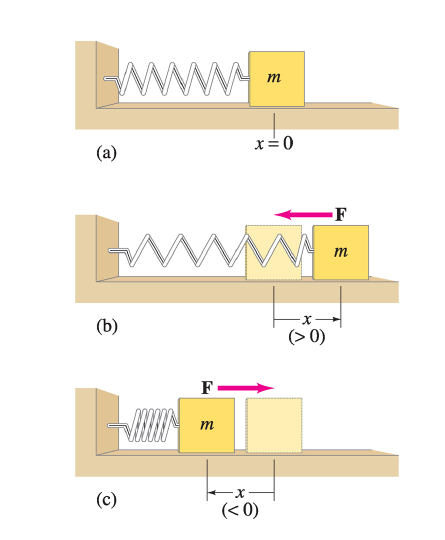
\includegraphics[width=4cm]{Grafik_Federpendel}
\centering
\caption{Federpendel [1]}
\centering
\end{figure}

Wird die Masse wie zuvor beschrieben ausgelenkt, also Energie zugeführt, und anschließend losgelassen, so schwingt das System um den Grundzustand. 
Über die Zeit betrachtet, führt die Masse eine Sinusschwingung aus, mit welcher sich allgemein Schwingungen beschreiben lassen:

\begin{align}
y(t) = \widehat{y} = sin(\omega_0 t )
\end{align}


Dabei ist $\widehat{y}$ die Amplitude, also die Auslenkung der Schwingung und $\omega_0$ die Kreisfrequenz mit welcher das System schwingt. 
Diese Berechnet sich aus der Frequenz, bzw. der Periodendauer [3]:

\begin{align}
T = \frac{1}{f}
\omega_0 = 2\pi \cdot f = \frac{2\pi}{T}
\end{align}

Für jedes schwingende System lässt sich eine Differentialgleichung aufstellen, mit welchem sich die verschiedenen wirkenden Kräfte beschreiben lassen. Für das lineare Feder-Masse-System ohne Dämpfung gilt: [2]

\begin{align}
F_a &= F_k &\\
\text{nach dem 2. Newtonsche Axiom gilt für die Masse:} F_a &= m \cdot a &\\
\text{und für die Federkraft das Hookesches Gesetz:} F_k &= -k \cdot y &
\end{align}

Durch einsetzen erhält man ein Gleichungssystem:

\begin{align}
-ky &= ma \\
m \frac{\partial y}{\partial t} + ky &= 0
\end{align}

Mit dem Ansatz $y(t) = \widehat{y_0} \cdot cos(\omega_0 t + \varphi_0)$ ergibt sich für das DGL.:

\begin{align}
\omega_0 = \sqrt{\dfrac{k}{m}}
\end{align}

Bei dem vorherigen System handelt es sich um eine freie ungedämpfe Schwingung. Diese gibt es in der Realität nur selten. Darum wird als nächstes die freie, gedämpfte Schwingung betrachtet.
Bei dieser wirkt eine Kraft, welche sich proportional zur Geschwindigkeit verhält und dem System Energie entzieht.

\begin{align}
F_D = -b \cdot v
\end{align}

Dabei ist b die Dämpfungskonstante. \\ 
Für die gedämpfte Schwingung lässt sich das DGL. um diesen Teil erweitern, wodurch sich folgendes Gleichungssystem ergibt.

\begin{align}
m \ddot{y} + d \dot{y} + k y = 0 
\end{align}

Der Ansatz für dises DGL. ist:

\begin{align}
y(t) = \widehat{y_0} e^{\delta t} cos(\omega_d t + \varphi_0)
\end{align}

Daraus als Lösung ergibt sich:

\begin{align}
\omega_d = \sqrt{\omega_0^2 - \delta^2} &\\
\delta = \dfrac{d}{2m} &\\
\omega_0 = \sqrt{\dfrac{k}{m}}
\end{align}

Dabei ist $\delta$ der Abklingkoeffizient. \\ \\

Abhängig von $\delta$ im Vergleich zu $\omega_0$ ergeben sich drei Fälle:

\textbf{Schwingfall:}\\
Wenn $\omega_0 > \delta$ schwingt das System mit abnehmender Amplitude und kann mit der Bewegungsgleichung

\begin{align}
y(t) = \widehat{y_0} e^{\delta t} cos(\omega_d t + \varphi_0)
\end{align}

beschrieben werden. [1]\\ 

\textbf{aperiodischer Genzfall:}\\
Wenn $\omega_0 = \delta$ schwingt das System nicht. Die Auslenkung strebt schnellstmöglich gegen Null. [1]\\

\textbf{Kriechfall:}\\
Wenn $\omega_0 < \delta$ schwingt das System ebenfalls nicht. Die Amplitude nimmt ganz langsam ab und erreicht asymptotisch die Null. [1]\\


Das folgende Diagramm zeigt das Verhalten bei den jeweiligen drei Fällen:

\begin{figure}[H]
\includegraphics[width=8cm]{Grafik_Fälle-Schwingungen}
\centering
\caption{Die drei Fälle der gedämpften Schwingung [1]}
\centering
\end{figure}

\subsection{Elektrischer Oszillator}
Der elektrische Oszillator ist dem mechanischen sehr ähnlich. Auch hier wird Ladungsenergie zwischen Kondensator und Spule stetig verschoben. Als Dämpfung wirkt der ohmsche Widerstand. 

In dem dargestellten Schwingkreis muss [3]:
\begin{align}
U_L + U_R + U_C = 0
\end{align}

Durch einsetzen der Strom- Spannungsabhängigkeiten für Widerstand, Spule und Kondensator [3]:
\begin{align}
U_L = L \cdot \frac{\partial i}{\partial t} &\\
U_C = \frac{1}{C} \cdot q &\\
U_R = R \cdot i &\\
\text{und:} \frac{\partial q}{\partial t} = i &
\end{align}

ergibt sich das DGL. [1]:
\begin{align}
L \cdot \frac{\partial^2 q}{\partial t^2} + R \cdot \frac{\partial q}{\partial t} + \frac{1}{c} \cdot q = 0
\end{align}

dessen Lösungen sind analog zu der mechanischen Schwingung [1]:
\begin{align}
\omega_d = \sqrt{\omega_0^2 - \delta^2} &\\
\delta = \dfrac{R}{2L} &\\
\omega_0 = \sqrt{\dfrac{1}{L \cdot C}}
\end{align}

\newpage

\section{Häusliche Vorarbeit}
\subsection{Mechanischer Oszillator}
\subsubsection{Aufgabe 3.1.1: Gleichung Rotationsschwinger}

\begin{align}
(m*\dfrac{d^2}{dt} + b*\dfrac{dx}{dt} + k*x = 0)
\end{align}

\begin{align*}
\text{Auslenkung:}& \quad x 							&&\longrightarrow \varphi \\
\text{Masse:}& \quad m   							&&\longrightarrow J \textit{(Trägheitsmoment)} &\\
\text{Geschwindigkeit:}& \quad v=\dfrac{dx}{dt} 		&&\longrightarrow \omega \textit{(Winkelgeschwindigeit)}&\\
\text{Beschleunigung:}& \quad a=\dfrac{d^2x}{dt^2} 	&&\longrightarrow \alpha \textit{(Winkelbeschleunigung)}&
\end{align*}

\begin{align*}
\text{Newton:}& \quad m \cdot a  		&&\longrightarrow J \cdot \alpha = J \dfrac{d\varphi}{dt} &\\
\text{Dämpfungsgrad:}& \quad b \cdot v  	&&\longrightarrow b \cdot \omega = b \dfrac{d^2\varphi}{dt^2} &\\
\text{Beschleunigung:}& \quad k \cdot x 	&&\longrightarrow k \cdot \varphi &
\end{align*}

\begin{align}
\Rightarrow \text{DGL.Torsionsschwinger:} \quad J*\dfrac{d^\varphi}{dt} + b*\dfrac{d\varphi}{dt} + k*\varphi = 0
\end{align}

\subsubsection{Aufgabe 3.1.2: Drehfederkonstante des Schwingers}

Definition Drehfederkonstante:
\begin{align}
M = k \cdot \varphi
\end{align}

Definition Drehmoment:
\begin{align}
M = r \cdot F
\end{align}

Aus Umstellen und Einsetzen der beiden Definitionen erhält man die Federkonstante aus Auslenkung und Kraft am Radius $r$:
\begin{align}
k = \dfrac{r \cdot F}{\varphi}
\end{align}

\begin{table}[H]
\begin{tabular}{|l|l|l|}
\hline
\textbf{$\varphi/rad$} & \textbf{$F/N$} & \textbf{$k/\dfrac{Nmm}{rad}$} \\ \hline
0,6                    & 0,1            & 15,83                         \\ \hline
0,8                    & 1,15           & 17,81                         \\ \hline
1,1                    & 0,2            & 17,27                         \\ \hline
1,3                    & 0,25           & 18,26                         \\ \hline
1,6                    & 0,3            & 17,81                         \\ \hline
1,8                    & 0,35           & 18,47                         \\ \hline
2,0                    & 0,4            & 19                            \\ \hline
2,3                    & 0,46           & 19                            \\ \hline
2,4                    & 0,48           & 19                            \\ \hline
\end{tabular}
\centering
\end{table}

Damit ergibt sich als Mittelwert die Federkonstante:

\begin{align*}
\Rightarrow \text{Federkonstante:} \quad \overline{k} \approx 18,1 \dfrac{Nmm}{rad} = 18,1 \cdot 10^{-3} \dfrac{Nm}{rad}
\end{align*}

\subsubsection{Aufgabe 3.1.3: Bestimmung der Massenträgheitsmomente}

\begin{align}
A_{ges} &= \Pi \cdot r^2 = 28352,87mm^2 \\
A_r &= A_{ges} - A_s = 24872,87mm^2 \\
m_r &= \dfrac{m_{ges}}{A_{ges} \cdot A_r = 22,47g}
\end{align}

Massenträgheitsmoment Hohlzylinder:
\begin{align}
J_r = \dfrac{1}{2} \cdot (r_{\textit{innen}}^2 + r_{\textit{außen}}^2) = 1629,59 kg \cdot mm^2
\end{align}

Massenträgheitsmoment Gesamt:
\begin{align}
J_{ges} = J_{s} + J_{r} = 1829,6 1629,59 kg \cdot mm^2 = 1829,6 \cdot 10^{-6} kg \cdot m^2
\end{align}
	
\subsubsection{Aufgabe 3.1.4: Berechnung der Eigenfrequenz}

Eigenfrequenz:
\begin{align}
\omega_{0,\textit{theor.}} = \sqrt{\dfrac{k}{J}} = 3,145 \dfrac{rad}{s}
\end{align}

Periodendauer:
\begin{align}
T_{0,\textit{theor.}} = \dfrac{2\Pi}{\omega_{0,\textit{theor.}}} = 1,99s
\end{align}

\subsection{Elektrischer Oszillator}
\subsubsection{Aufgabe 3.2.1: Ersatzwiderstand der Spule}

Eine Spule besteht aus einem (dünnen) gewickelten Draht, welcher selbst einen Leitungswiederstand aufweist.
Dieser kann ersatzweise als Widerstand in Reihe zu der Spule dargestellt werden.

\subsubsection{Aufgabe 3.2.2: Gesamtwiderstand}

bei dem Gesamtwiederstand handelt es sich um eine Reihenschaltung aus dem Innenwiderstand der Spule und den beiden externen Widerständen. 
\begin{align}
R_{ges} = R_1 + R_2 + R_3
\end{align}

Als Ungenauigkeit der externen Widerstände wird $\mp 0,05 k \Omega$ angenommen.

\begin{align*}
R_{3,min} = (0+0,05)k\Omega &\Rightarrow R_{ges,min} = (6,45+0,1)k\Omega \\
R_{3,max} = (10\mp0,05)k\Omega &\Rightarrow R_{ges,min} = (16,45\mp0,1)k\Omega
\end{align*}

\subsubsection{Aufgabe 3.2.3: Eigenfrequenz ohne Dämpfung}

\begin{align}
\omega_{0,\textit{theor.}} = \sqrt{\dfrac{1}{LC}}= 1497,8318 \frac{1}{s}
\end{align}

Fehlerrechnung:
\begin{align*}
\vert \frac{\partial}{\partial L}\omega_{0,\textit{theor.}}\vert = \frac{LC}{2L^2C} &\\
\vert \frac{\partial}{\partial C}\omega_{0,\textit{theor.}}\vert = \frac{LC}{2LC^2} &
\end{align*}
\begin{align*}
U_{\omega_{0,\textit{theor.}}} = \vert \frac{\partial}{\partial L}\omega_{0,\textit{theor.}}\vert \cdot U_L + \vert \frac{\partial}{\partial C}\omega_{0,\textit{theor.}}\vert \cdot U_C = 140,841 \frac{rad}{s} \approx 150 \frac{1}{s}
\end{align*}

\begin{align*}
\Rightarrow \omega_{0,\textit{theor.}} = (1490 \mp 150) \frac{1}{s}
\end{align*}

\subsubsection{Aufgabe 3.2.4: Abklingkoeffizient}

\begin{align}
\delta_{\textit{theor.}} = \dfrac{R}{2L}= 151,3453 \frac{1}{s}
\end{align}

Fehlerrechnung:
\begin{align*}
\vert \frac{\partial}{\partial R}\delta_{\textit{theor.}}\vert = \frac{1}{2L} &\\
\vert \frac{\partial}{\partial L}\delta_{\textit{theor.}}\vert = \frac{R}{2L^2} &
\end{align*}
\begin{align*}
U_{\delta_{\textit{theor.}}} = \vert \frac{\partial}{\partial R}\delta_{\textit{theor.}}\vert \cdot U_R + \vert \frac{\partial}{\partial L}\delta_{\textit{theor.}}\vert \cdot U_L = 11,4863 \approx 12  \frac{1}{s}
\end{align*}

\begin{align*}
\Rightarrow \delta_{\textit{theor.}} = (151 \mp 12) \frac{1}{s}
\end{align*}

\subsubsection{Aufgabe 3.2.5: gedämpfte Eigenfrequenz}

\begin{align}
\omega_{D,\textit{theor.}} = \sqrt{\omega_{0,\textit{theor.}}^2 - \delta_{\textit{theor.}}^2} = 1482,329 \frac{1}{s}
\end{align}

Fehlerrechnung:
\begin{align*}
\vert \frac{\partial}{\partial \omega_{0,\textit{theor.}}}\omega_{D,\textit{theor.}}\vert = \frac{\omega_{0,\textit{theor.}}}{\sqrt{\omega_{0,\textit{theor.}}^2 - \delta_{\textit{theor.}}^2}} &\\
\vert \frac{\partial}{\partial \delta_{\textit{theor.}}}\omega_{D,\textit{theor.}}\vert = \frac{\delta_{\textit{theor.}}}{\sqrt{\omega_{0,\textit{theor.}}^2 - \delta_{\textit{theor.}}^2}} &
\end{align*}
\begin{align*}
U_{\omega_{D,\textit{theor.}}} = \vert \frac{\partial}{\partial \omega_{0,\textit{theor.}}}\omega_{D,\textit{theor.}}\vert \cdot U_{\omega_{0,\textit{theor.}}} + \vert \frac{\partial}{\partial \delta_{\textit{theor.}}}\omega_{D,\textit{theor.}}\vert \cdot U_{\delta_{\textit{theor.}}} = 151,9716 \approx 160 \frac{1}{s}
\end{align*}

\begin{align*}
\Rightarrow \omega_{D,\textit{theor.}} = (1480 \mp 160) \frac{1}{s}
\end{align*}

\subsubsection{Aufgabe 3.2.6: Gesamtwiderstand beim aperiodischer Grenzfall}

Bedingung für den aperiodischer Grenzfall:
\begin{align}
\text{Aperiodicher Genzfall:} \quad \omega_{0,\textit{theor.}}^2 = \delta_{\textit{theor.}}^2
\end{align}

\begin{align*}
(\omega_{0,\textit{theor.}} \text{ist unabhängig von R}) \quad \text{und} \quad
\delta_{\textit{theor.}} = \frac{R}{2L}
\end{align*}

damit ergibt sich als Gleichung zur Bestimmung des Widerstandes:

\begin{align}
\omega_{0,\textit{theor.}}^2 = \frac{R^2}{4L^2} \quad \Rightarrow \quad R_{\textit{grenz,theor.}} &= \omega_{0,\textit{theor.}} \cdot 2L = 13290,8 \Omega
\end{align}


Fehlerrechnung:
\begin{align*}
\vert \frac{\partial}{\partial \omega_{0,\textit{theor.}}}R_{\textit{grenz,theor.}}\vert = 2 \cdot L &\\
\vert \frac{\partial}{\partial L}R_{\textit{grenz,theor.}}\vert = 2 \cdot \omega_{0,\textit{theor.}} &
\end{align*}
\begin{align*}
U_{R_{\textit{grenz,theor.}}} = \vert \frac{\partial}{\partial \omega_{0,\textit{theor.}}}R_{\textit{grenz,theor.}}\vert \cdot U_{\omega_{0,\textit{theor.}}} + \vert \frac{\partial}{\partial L}R_{\textit{grenz,theor.}}\vert \cdot U_L = 1840,60 \approx 1900 
\end{align*}

\begin{align*}
\Rightarrow R_{\textit{grenz,theor.}} = (13,3 \mp 1,9) k \Omega
\end{align*}

\subsubsection{Aufgabe 3.2.6: Funktion des Tasters}
Der Taster verbindet in seiner Ausgangspostion die Spannungsquelle mit dem Kondensator, sodass dieser geladen wird und so der Schwingung ihre Startenergie zugeführt wird. Wird der Taster betätigt, wird die Spannungsversorgung getrennt und der Schwingkreis aus Widerstand, Spule und Kondensator geschlossen, wodurch eine freie gedämpfte Schwingung zwischen Spule und Kondensator stattfindet. Dabei oszilliert die zuvor dem Kondensator zugeführte Energie zwischen den beiden Bauteilen.

\newpage

\section{Aufbau und Durchführung}
\subsection{Mechanischer Oszillator}
\subsubsection{Aufbau}
Bei dem mechanischen Oszillator, handelt es sich um das Pohlsche Rad.
Der Aufbau besteht aus einem Reibungsfrei gelagertem Rad mit einer bestimmten Masse.
Mit einer Spiralfeder um die Achse ist das Rad an dem Ursprung befestigt.
Die Auslenkung des Rades wird mit einem digitalen Oszilloskop abgelesen.
Zusätzlich kann das Rad durch eine Wirbelstrombremse gebremst, bzw. die Schwingung gedämpft werden.

\begin{figure}[H]
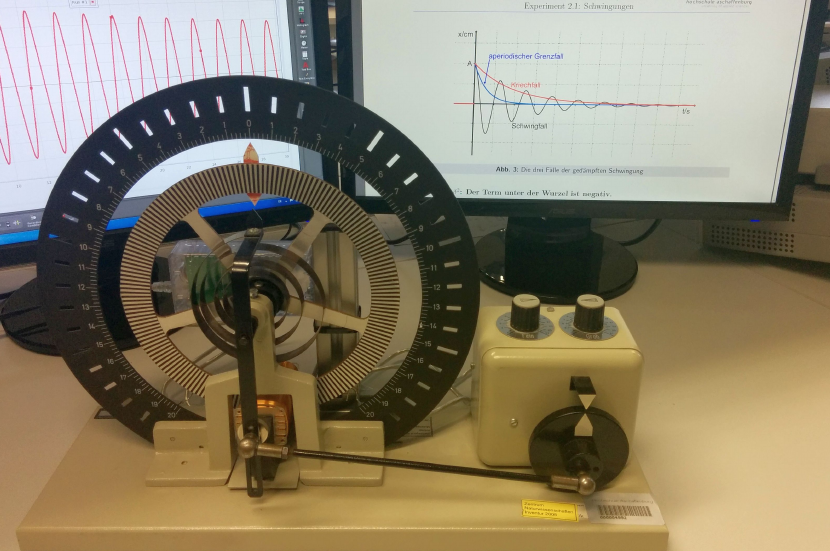
\includegraphics[width=10cm]{Grafik_Pholsches-Rad}
\centering
\caption{Versuchsaufbau (Pohlsches Rad) [1]}
\centering
\end{figure}

\subsubsection{Durchführung}
Zunächst wird die Aufnahme mit dem digitalen Oszilloskop gestartet, danach wird der
Zeiger des Rades nach links ausgelenkt und so Anfangsenergie zugefügt. Anschließend wird das Rad losgelassen und das System sich selbst überlassen. Der Versuch wird für verschiedene Bremsströme wiederholt.

\subsection{Elektrischer Oszillator}
\subsubsection{Aufbau}
Die folgende Schaltung wird auf einem Steckbrett aufgebaut:

\begin{figure}[H]
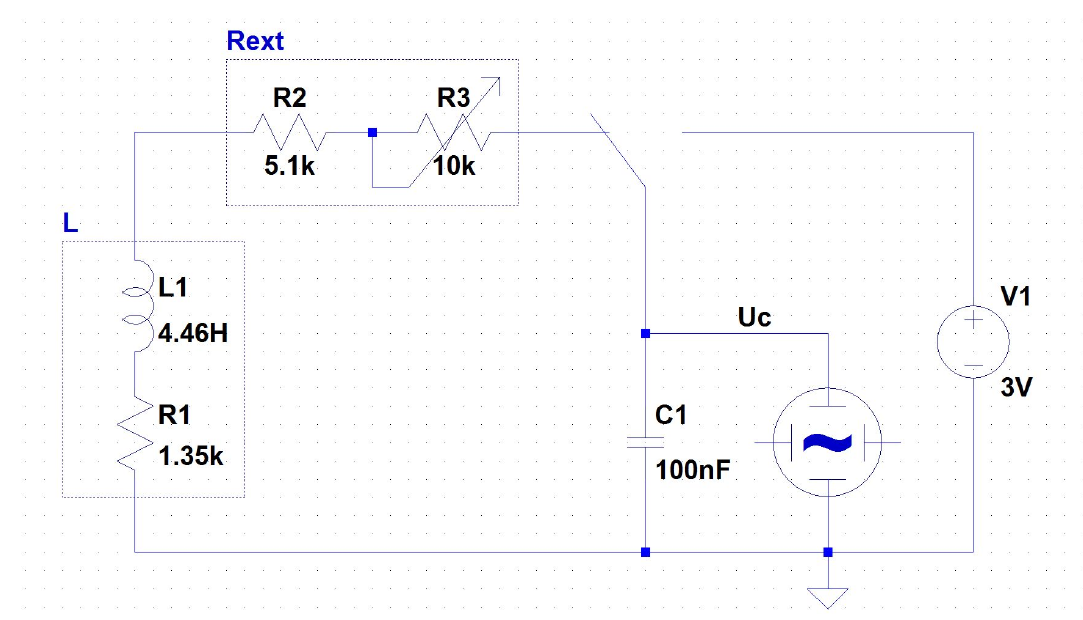
\includegraphics[width=9cm]{Grafik_el-Oszillator}
\centering
\caption{Versuchsaufbau elektrischer Oszillator [1]}
\centering
\end{figure}

\subsubsection{Durchführung}
Im ersten Versuchsdurchlauf werden die externen Widerstände überbrückt. Durch betätigen des Tasters wird eine freie Schwingung ermöglicht, welche an dem Oszilloskop zu sehen ist.
Im zweiten Teil des Versuches wird die Brücke über die Widerstände entfernt. Nun wird durch mehrfaches betätigen des Tasters und beobachten des Ergebnisses, während man mit dem Potentiometer den Widerstand verändert, der aperiodische Grenzfall eingestellt. 
Anschließend wird der Widerstand, bei welchem der Fall erreicht wurde, gemessen.

\newpage

\section{Auswertung Versuch}
\subsection{Mechanischer Oszillator}
Im folgenden werden die Messergebnisse für den Versuch mit den vier verschiedenen Bremsströmen ausgewertet. Da zuerst das Rad zu Beginn des Versuches ausgelenkt werden muss und so die freie Schwingung erst ab einem bestimmten Zeitpunkt vorlag, wird in den jeweiligen Diagrammen der Zeitpunkt markiert, ab welchem diese freie Schwingung vorlag.

\subsubsection{Bremsstrom 0A - freie Schwingung}
Bei der ersten Durchführung war der Strom der Wirbelstrombremse vollständig abgeschaltet, um einen möglichst ungedämpften Fall zu erreichen.

\begin{figure}[H]
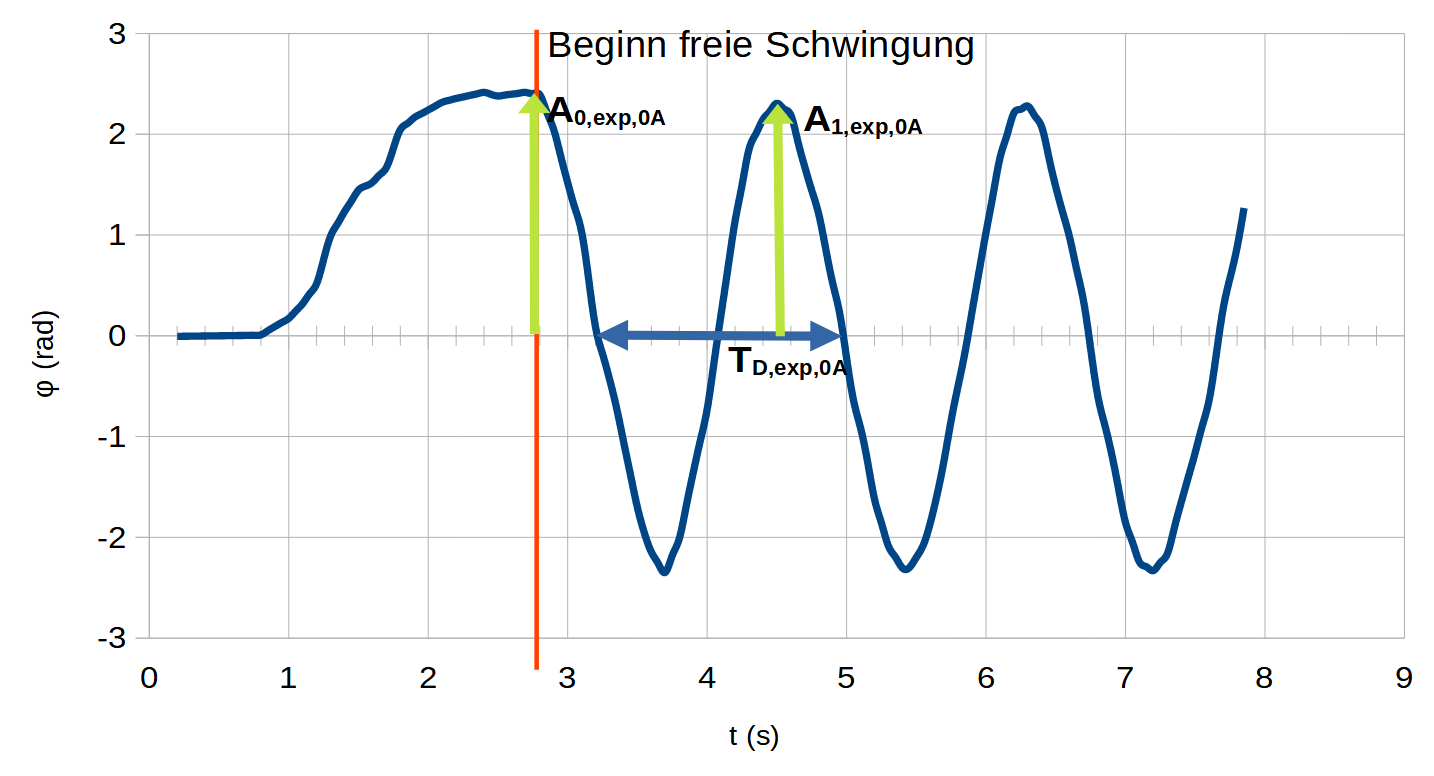
\includegraphics[width=8cm]{Messung_Rad_graph_0A}
\centering
\caption{Messung Pohlsches Rad 0A}
\centering
\end{figure}

Bei dem Versuchsdurchlauf handelt es sich, um eine freie Schwingung. Die Schwingung verläuft periodisch und die Amplitude nimmt nur wenig (durch den Luftwiederstand und Reibung in den Lagern ist keine vollständig ungedämpfte Schwingung möglich) ab, wodurch die Schwingung ungedämpft ist.
\\ \\
\textbf{Aus dem Diagramm lässt sich ablesen:}
\begin{align*}
\text{Periodendauer:} T_{0,\textit{exp.},0A} = (1,80\mp0,10)s \\
\end{align*}
Der Abklingkoeffizient kann nicht genau aus den Messdaten abgelesen werden, da die Dämpfung zu klein und somit $A_{0,\textit{exp.},0A} \approx A_{1,\textit{exp.},0A}$ ist
\\ \\
\textbf{Berechnung der Kreisfrequenz:}
\begin{align}
\omega_{0,\textit{exp.},0A} = \frac{2\pi}{T_{0,\textit{exp.},0A}} = 3,496 \frac{1}{s}
\end{align}

Mit dem theoretischen Wert von $\omega_{0,\textit{theor.}} = 3,145 \dfrac{1}{s}$ verglichen ist die Abweichung eher gering. Der Versuch kann somit als gut betrachtet werden.


\subsubsection{Bremsstrom 0,5A - gedämpfte Schwingung}
Bei der zweiten Durchführung war der Strom der Wirbelstrombremse auf $I = 0,498A$ eingestellt, um eine leichte Dämpfung zu erreichen.

\begin{figure}[H]
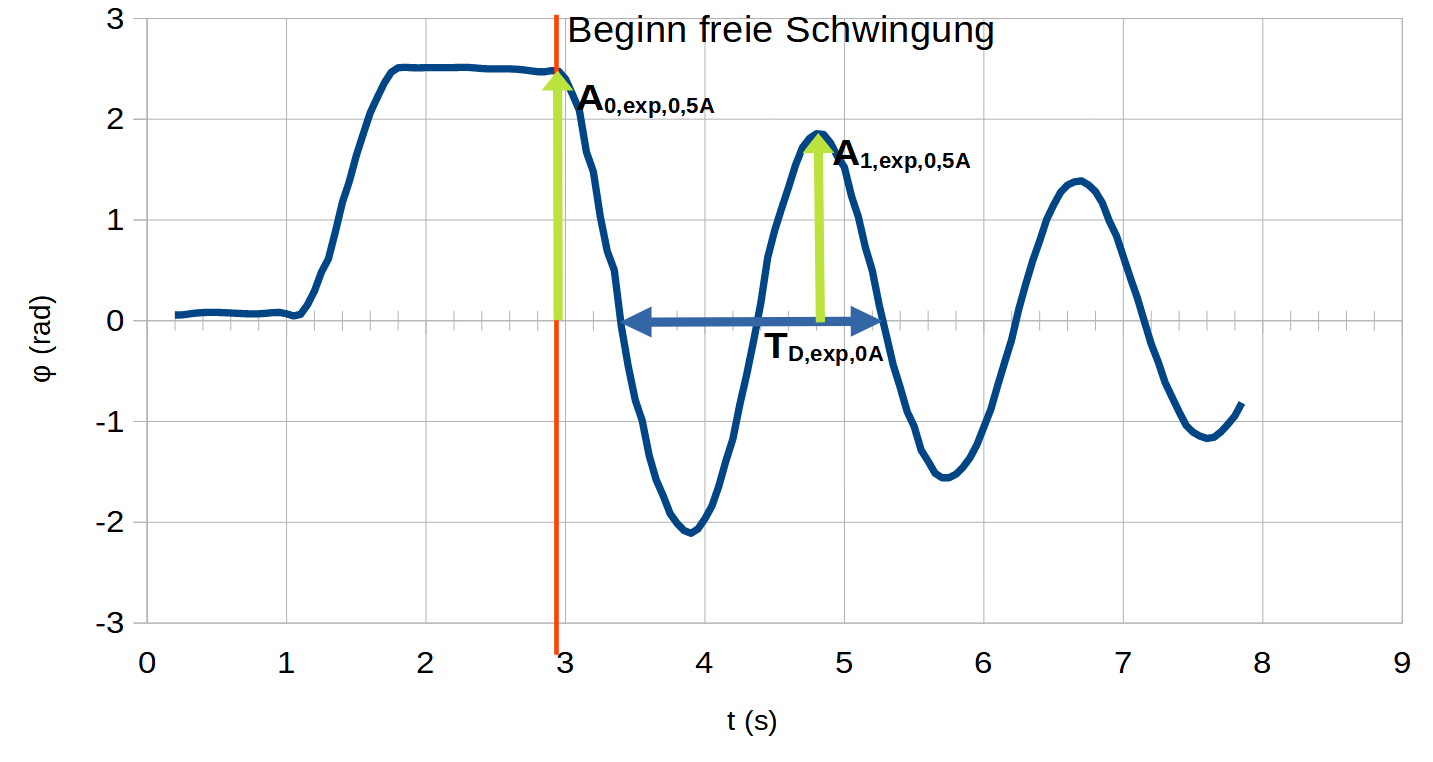
\includegraphics[width=8cm]{Messung_Rad_graph_05A}
\centering
\caption{Messung Pohlsches Rad 0,5A}
\centering
\end{figure}

Bei dem Versuchsdurchlauf handelt es sich um eine gedämpfte Schwingung. Die Schwingung verläuft periodisch und die Amplitude nimmt fortlaufend exponentiell ab, wodurch die Schwingung gedämpft ist.
\\ \\
\textbf{Aus dem Diagramm lässt sich ablesen:}

\begin{align*}
\text{Periodendauer:} T_{D,\textit{exp.},0A} = (1,90\mp0,10)s \\
\text{Auslenkung 0. Maxima:} A_{0,\textit{exp.},0,5A} = (2,5\mp0,2)rad \\
\text{Auslenkung 1. Maxima:} A_{1,\textit{exp.},0,5A} = (1,9\mp0,2)rad
\end{align*}

Da die Daten des Diagramms nicht genau exportiert werden konnten und anhand eines abfotografierten Bildes ermittelt wurden, ist eine sehr große Ungenauigkeit vorhanden. \\

\textbf{Berechnung der gedämpften Kreisfrequenz:}
\begin{align}
\omega_{D,\textit{exp.},0,5A} = \frac{2\pi}{T_{D,\textit{exp.},0,5A}} = 3,31 \frac{1}{s}
\end{align}

\textbf{Berechnung des Logarithmischen Dekrements:}

\begin{align}
\Lambda_{\textit{exp.},0,5A} = \ln(\frac{A_{0,\textit{exp.},0,5A}}{A_{1,\textit{exp.},0,5A}}) = 0,51
\end{align}

\textbf{Berechnung des Abklingkoeffizienten:}

\begin{align}
\delta_{\textit{exp.},0,5A} = \frac{\Lambda_{\textit{exp.},0,5A}}{T_{D,\textit{exp.},0,5A}} = 0,27 \frac{1}{s}
\end{align}

\textbf{Berechnung der Kreisfrequenz des ungedämpften Systems:}

\begin{align}
\omega_{0,\textit{exp.},0,5A} = \sqrt{\omega_{D,\textit{exp.},0,5A}^2 + \delta_{\textit{exp.},0,5A}^2} = 3,32 \frac{1}{s}
\end{align}

Mit dem theoretischen Wert von $\omega_{0,\textit{theor.}} = 3,145 \dfrac{1}{s}$ verglichen ist eine eher große Abweichung zu erkennen. Diese geht zum größten Teil auf die oben bereits erwähnten Abweichungen beim Ablesen zurück.

\subsubsection{Bremsstrom 2,1A - aperiodischer Grenzfall}
Bei der dritten Durchführung war der Strom der Wirbelstrombremse auf $I = 2,201$ eingestellt, um so möglichst genau den aperiodischer Grenzfall zu treffen.

\begin{figure}[H]
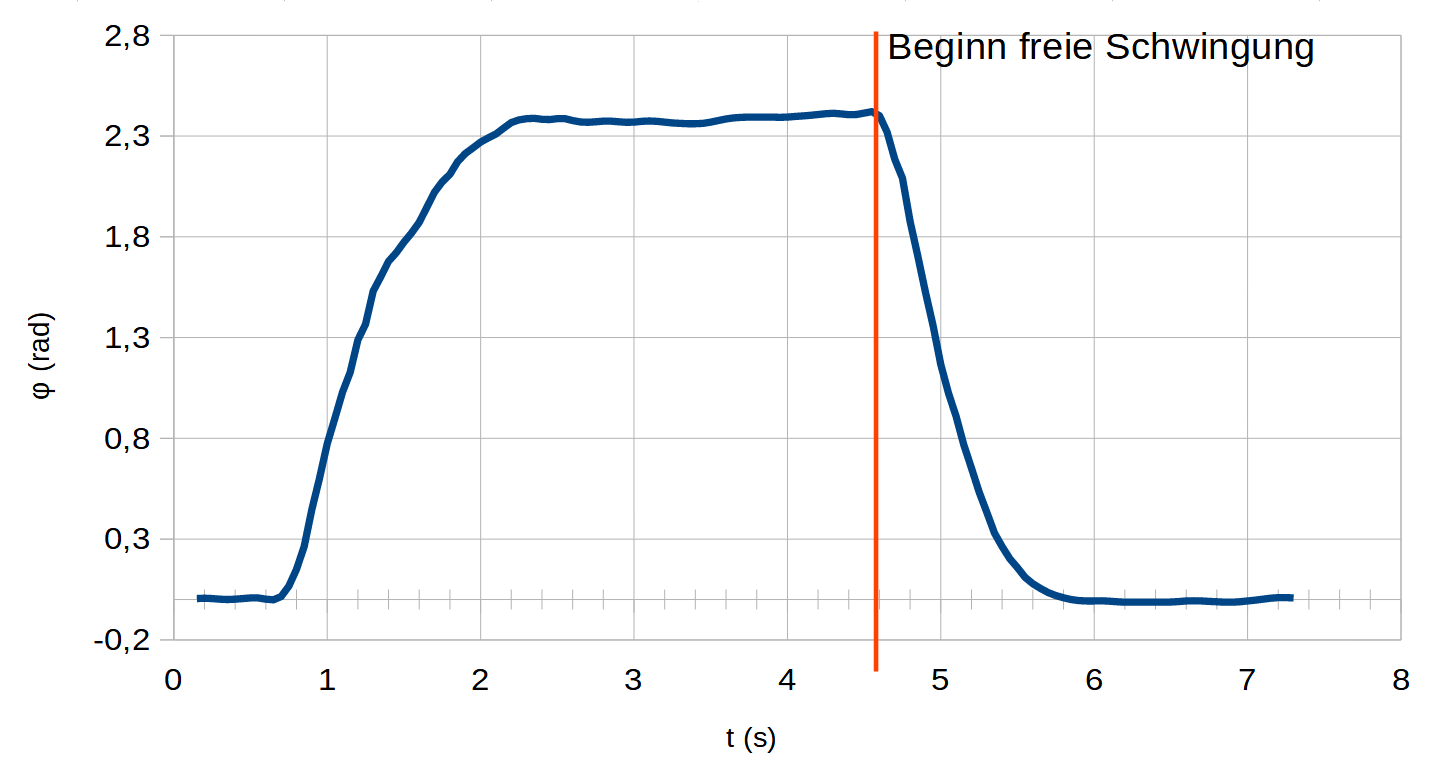
\includegraphics[width=8cm]{Messung_Rad_graph_21A}
\centering
\caption{Messung Pohlsches Rad 2,1A}
\centering
\end{figure}

Bei dem Versuchsdurchlauf handelt es sich um den aperiodischen Grenzfall. Die Schwingung ist so stark gedämpft, dass diese bereits nach einer halben Schwingung zum Stillstand kommt. Dabei beginnt die Schwingung, wie die ungedämpfte Schwingung, nähert sich dann jedoch der null Position an, ohne in negative Richtung über zu schwingen. 

\subsubsection{Bremsstrom 2,5A - Kriechfall}
Bei der vierten Durchführung war der Strom der Wirbelstrombremse auf $I = 2,515$ eingestellt, um so eine möglichst große Dämpfung zu erreichen.

\begin{figure}[H]
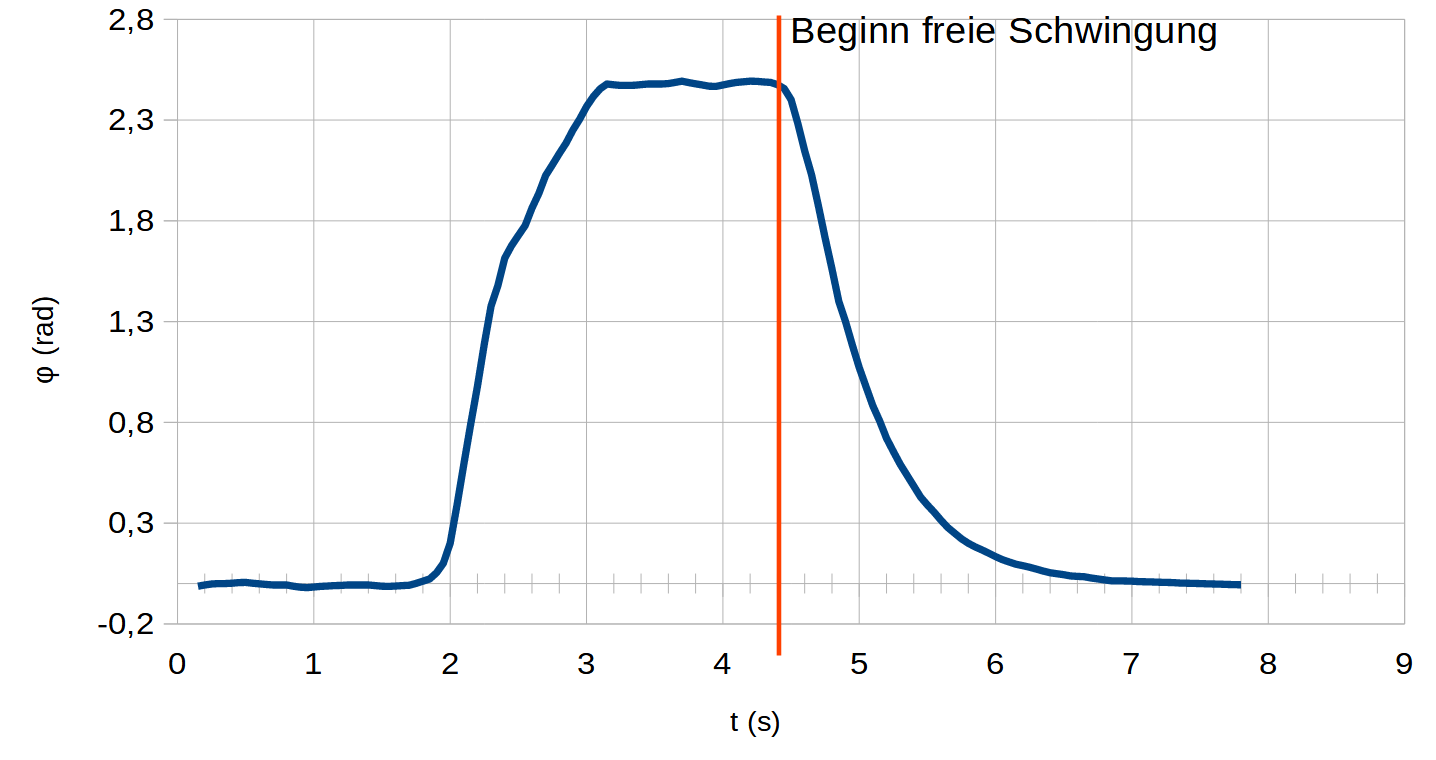
\includegraphics[width=8cm]{Messung_Rad_graph_25A}
\centering
\caption{Messung Pohlsches Rad 2,5A}
\centering
\end{figure}

Bei dem Versuchsdurchlauf handelt es sich um den aperiodischen Grenzfall. Die Schwingung ist so stark gedämpft, kein schwingendes Verhalten zu erkennen ist. Dabei nähert sich das Rad seiner null Position nur langsam asymptotisch an. 

\subsubsection{Gegenüberstellung Tabelle}
Die gemessenen und theoretischen Werte können in einer Tabelle gegenüber gestellt werden.

\begin{table}[H]
\begin{tabular}{|l|l|l|l|}
\hline
 									& \textbf{Theorie} & \textbf{Experiment 1} & \textbf{Experiment 2} \\ \hline
\textbf{$\omega_0$ in $\frac{1}{s}$} & 3,145            & 3,496                 & 3,32       	         \\ \hline
\textbf{$T_0$ in $s$}                & 1,99             & 1,80                  & 1,89        			 \\ \hline
\textbf{$\omega_D$ in $\frac{1}{s}$} & /                & /                     & 3,31        			 \\ \hline
\textbf{$T_D$ in $s$}                & /                & /                     & 1,90        			 \\ \hline
\end{tabular}
\centering
\end{table}

\subsection{Elektrischer Oszillator}
Im folgenden werden die Messergebnisse für den Versuch des elektrischen Oszillators ausgewertet. Bei dem ersten Durchgang wurden sämtliche externen Widerstände überbrückt, um eine möglichst ungedämpfte Schwingung zu erreichen. Bei dem zweiten Versuch wurde Näherungsweise versucht, genau den aperiodischen Grenzfall, mit Hilfe eines Potentiometers, einzustellen.

\subsubsection{Schwingfall}

\begin{figure}[H]
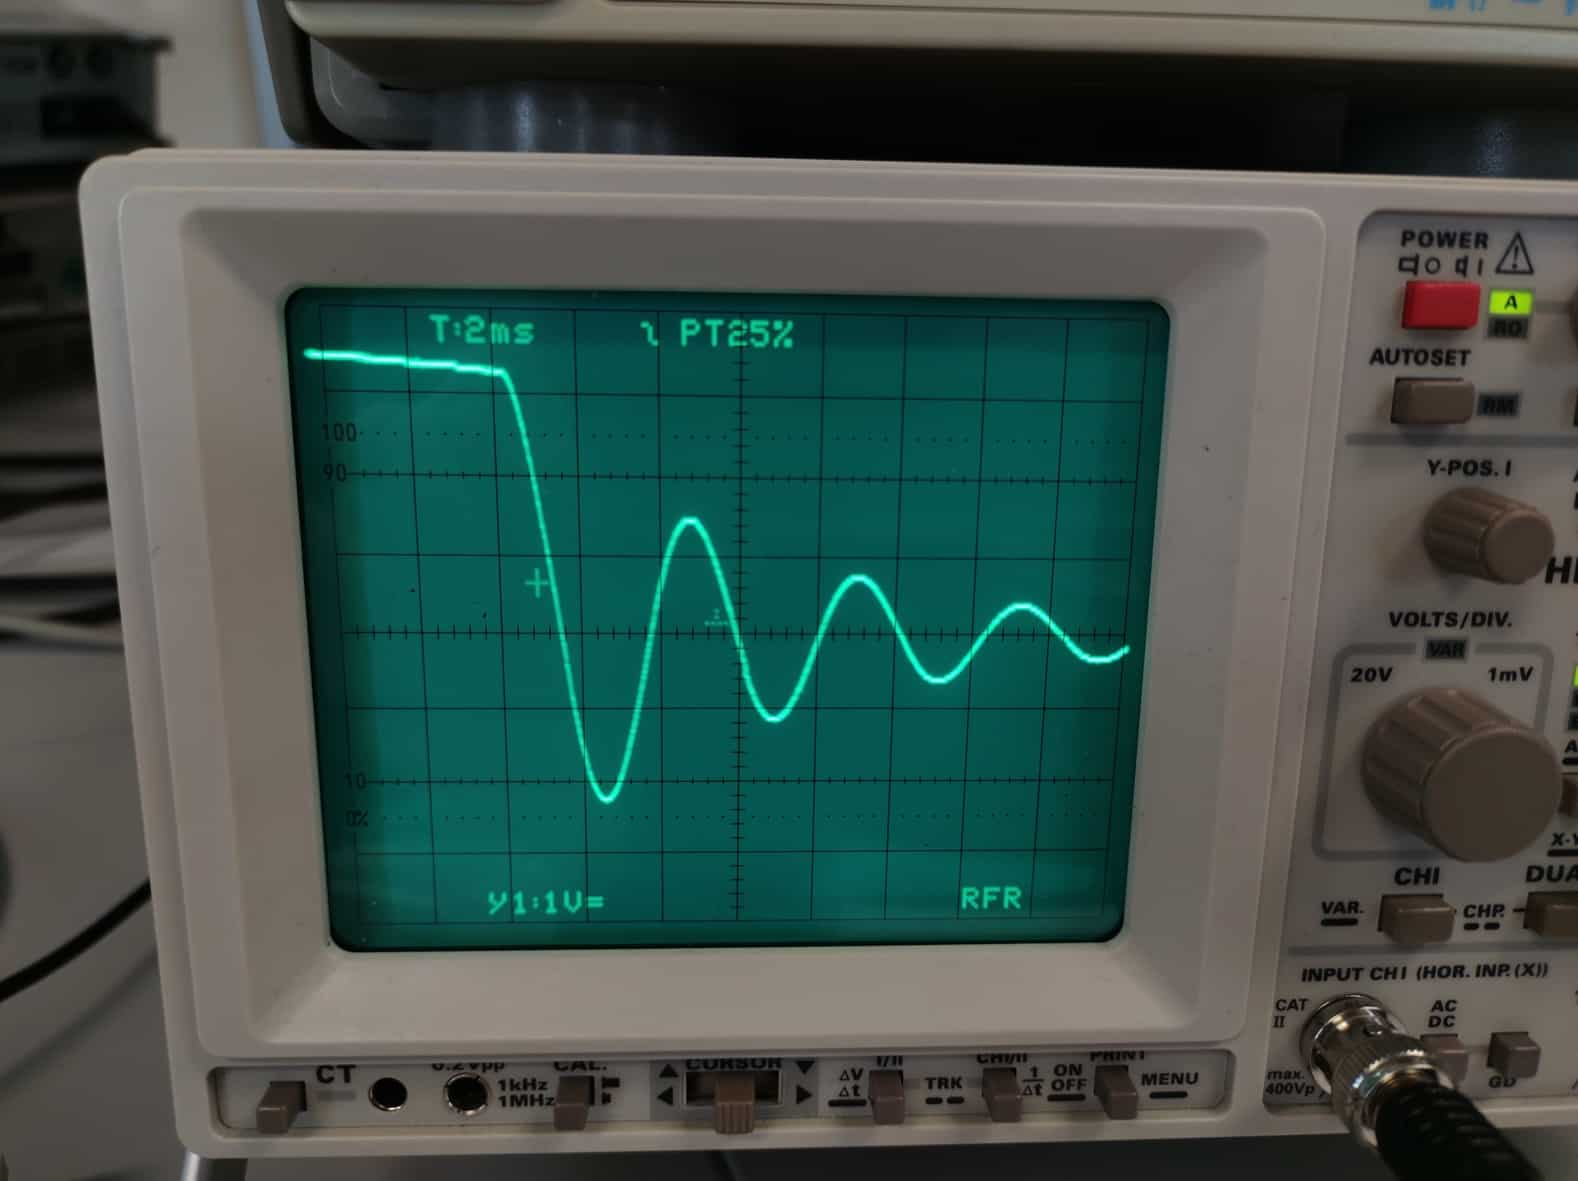
\includegraphics[width=8cm]{Bild_Osziloskop-Schwingung}
\centering
\caption{Osziloskop: Schwingfall}
\centering
\end{figure}

\textbf{Aus dem Diagramm lässt sich ablesen:}
\begin{align*}
T_{D,\textit{exp.}} = (4,4\mp0,1)ms \\
A_{0,\textit{exp.}} = (3,2\mp0,1)V \\
A_{1,\textit{exp.}} = (1,5\mp0,1)V
\end{align*}

\textbf{Kreisfrequenz der gedämpften Schwingung:}
\begin{align}
\omega_{D,\textit{exp.}} = \frac{2\pi}{T_{D,\textit{exp.}}} = 1427,997 \frac{1}{s}
\end{align}

Fehlerrechnung:
\begin{align*}
\vert \frac{\partial}{\partial T_{D,\textit{exp.}}}\omega_{D,\textit{exp.}}\vert = \frac{2\pi}{T_{D,\textit{exp.}}^2}
\end{align*}
\begin{align*}
U_{\omega_{D,\textit{exp.}}} = \vert \frac{\partial}{\partial T_{D,\textit{exp.}}}\omega_{D,\textit{exp.}}\vert \cdot U_{T_{D,\textit{exp.}}} = 32,45 \approx 33 \frac{1}{s} 
\end{align*}

\begin{align*}
\Rightarrow \omega_{D,\textit{exp.}} = (1428 \mp 33) \frac{1}{s}
\end{align*}

Mit dem theoretischen Wert von $\omega_{D,\textit{theor.}} = (1480\mp160) \frac{1}{s}$ verglichen, ist der Wert nur knapp nicht innerhalb der für den Versuch bei der Messung angenommenen Messunsicherheiten. Wenn man die theoretische Messunsicherheit betrachtet, welche den nicht genauen Spulen-Widerstand berücksichtigt (die gemessene Unsicherheit berücksichtigt nur die, durch Messungsfehler entstehenden Abweichungen), ist das tatsächliche Messergebiss innerhalb der Messunsicherheit, womit das Ergebnis akzeptabel ist.

\textbf{Berechnung des logarithmischen Dekrements:}
\begin{align}
\Lambda_{\textit{exp.}} = ln(\frac{A_{0,\textit{exp.}}}{A_{1,\textit{exp.}}}) = 0,7576
\end{align}

Fehlerrechnung:
\begin{align*}
\vert \frac{\partial}{\partial A_{0,\textit{exp.}}}\Lambda_{\textit{exp.}}\vert = \frac{1}{A_{0,\textit{exp.}}} \\
\vert \frac{\partial}{\partial A_{1,\textit{exp.}}}\Lambda_{\textit{exp.}}\vert = \frac{1}{A_{1,\textit{exp.}}}
\end{align*}

\begin{align*}
U_{\Lambda_{\textit{exp.}}} = \vert \frac{\partial}{\partial A_{0,\textit{exp.}}}\Lambda_{\textit{exp.}}\vert \cdot U_{A_{0,\textit{exp.}}} + \vert \frac{\partial}{\partial A_{1,\textit{exp.}}}\Lambda_{\textit{exp.}}\vert \cdot U_{A_{1,\textit{exp.}}} = 0,07569 \approx 0,076 
\end{align*}

\begin{align*}
\Rightarrow \Lambda_{\textit{exp.}} = (0,758 \mp 0,076)
\end{align*}

\textbf{Berechnung des Abklingkoeffizienten:}
\begin{align}
\delta_{\textit{exp.}} = \frac{\Lambda_{\textit{exp.}}}{T_{D,\textit{exp.}}} = 172,1818 \frac{1}{s}
\end{align}

Fehlerrechnung:
\begin{align*}
\vert \frac{\partial}{\partial \Lambda_{\textit{exp.}}}\delta_{\textit{exp.}}\vert = \frac{1}{T_{D,\textit{exp.}}} \\
\vert \frac{\partial}{\partial T_{D,\textit{exp.}}}\delta_{\textit{exp.}}\vert = \frac{\Lambda_{\textit{exp.}}}{T_{D,\textit{exp.}}^2}
\end{align*}

\begin{align*}
U_{\delta_{\textit{exp.}}} = \vert \frac{\partial}{\partial \Lambda_{\textit{exp.}}}\delta_{\textit{exp.}}\vert \cdot U_{\Lambda_{\textit{exp.}}} + \vert \frac{\partial}{\partial T_{D,\textit{exp.}}}\delta_{\textit{exp.}}\vert \cdot U_{T_{D,\textit{exp.}}} = 21,1859 \approx 22 \frac{1}{s}
\end{align*}

\begin{align*}
\Rightarrow \delta_{\textit{exp.}} = (172 \mp 22) \frac{1}{s}
\end{align*}

Mit dem theoretischen Wert von $\delta_{\textit{theor.}} = (151 \mp 12) \frac{1}{s}$ verglichen, bewegt sich das Ergebiss knapp innerhalb der Messunsicherheiten und ist somit als gut zu betrachten.



\subsubsection{Aperiodischer Grenzfall}

\begin{figure}[H]
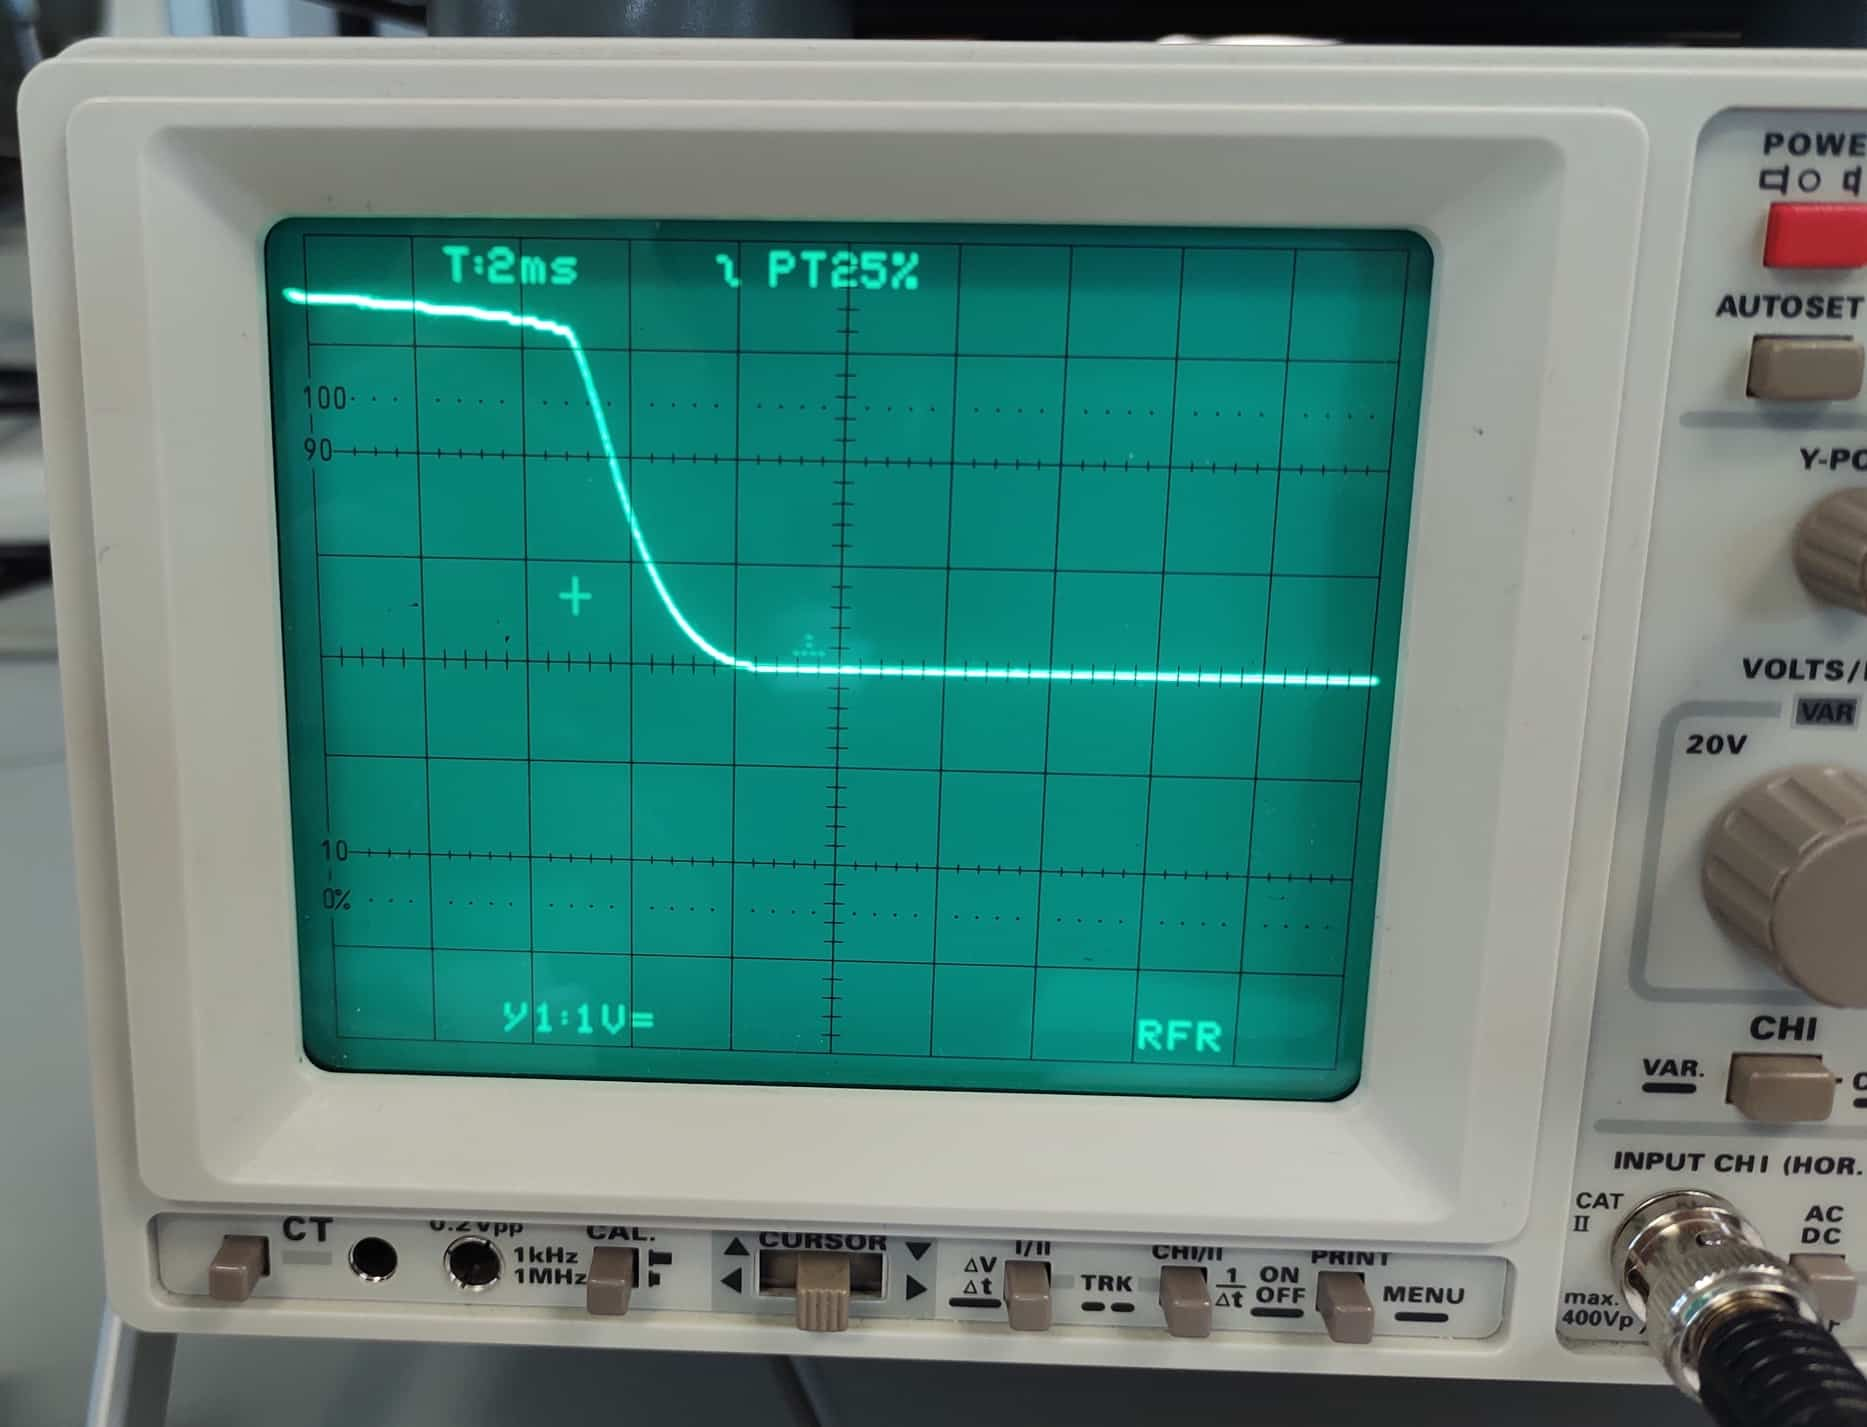
\includegraphics[width=8cm]{Bild_Osziloskop-Grenzfall}
\centering
\caption{Osziloskop: Aperiodischer Grenzfall}
\centering
\end{figure}

\textbf{Aus dem Diagramm lässt sich ablesen:}
\begin{align*}
R_{\textit{ext,exp.}} = (10,084\mp2,0)k\Omega
\end{align*}
Dabei wird als Messungenauigkeit $2k\Omega$ angenommen. Die Ungenauigkeit entsteht vor allem dadurch, dass sich der Widerstand in diesem Bereich verändern lässt, ohne, dass an dem Oszilloskop eine wesentlich Änderung erkennbar ist. Es ist also schwer zu erkennen, wann genau der Grenzfall eintritt.
Die Messunsicherheit des Ohrmeters wird von diesem Faktor überschattet und ist irrelevant.

\textbf{Berechnung Gesamtwiderstand:}
\begin{align}
R_{\textit{ges,exp.}} = R_{\textit{ext,exp.}} + R_{\textit{int,exp.}} = 11,434k\Omega 
\end{align}

Fehlerrechnung:
\begin{align*}
U_{R_{\textit{ges,exp.}}} = U_{R_{\textit{ext,exp.}}} + U_{R_{\textit{int,exp.}}} = 2,051k\Omega \approx 2,0k\Omega
\end{align*}

\begin{align*}
\Rightarrow R_{\textit{ges,exp.}} = (11,4 \mp 2,0) k\Omega
\end{align*}

Mit dem theoretischen Wert von $R_{\textit{grenz,theor.}} = (13,3 \mp 1,9)k \Omega$ verglichen, ist das Ergebnis innerhalb der für den Versuch angenommenen Messunsicherheiten. Wie bereits zu Beginn erwähnt, ist es schwierig genau den aperiodischen Fall auf dem Oszilloskop zu bestimmen, das der Übergang zwischen den verschiedenen Fällen fließend ist. Selbst wenn man den genauen Wert als Hilfe nehmen würde, ist es fragwürdig, ob die Änderung auf den Oszilloskop zu erkennen gewesen wäre.

\newpage

\section{Wertung/Fazit}
\subsection{Mechanischer Oszillator}
Bei der Durchführung des Versuches ließen sich die verschieden Fälle, der Schwing-, Grenz- und Kriechfall, deutlich erkennen. Die, bei der Auswertung ergebenen Werte, stimmen gut mit der Theorie überein, obwohl die Abweichungen teilweise sehr groß sind. In den jeweiligen Fällen wurden die erkannten Probleme bereits erläutert.

\subsection{Elektrischer Oszillator}
Beim elektrischen Oszillator waren ebenfalls die drei unterschiedlichen Fälle, die bei Schwingungen auftreten können, gut sichtbar. Bei der Bestimmung des Grenzfalls wurde mit Augenmaß entschieden, ab wann es sich um einen aperiodischen Grenzfall handelt. Deswegen sind beim Vergleichen der Messergebnisse von dem Experiment mit der Theorie deutliche Differenzen festgestellt worden, bzw. die Messunsicherheit wurde bereits vor der Auswertung sehr groß geschätzt.
Auch lag bei der ungedämpften Schwingung aufgrund des unvermeidbaren Spulenwiderstandes eine bereits sehr große Dämpfung vor.

\newpage

\section{Literatur}
$[$1$]$ Skript: Versuch 2.1 - Schwingungen \\
$[$2$]$ Vorlesungsfolien: 1. Semester Physik, Herr Prof. Kaloudis \\
$[$3$]$ Hering, Ekbert ; Martin, Rolf ; Stohrer, Martin: Physik für Ingenieure. Springer-Verlag

\label{LastPage}

\end{document}
%%% Local Variables:
%%% mode: latex
%%% TeX-master: t
%%% End: